\begin{figure}[H]
\centering
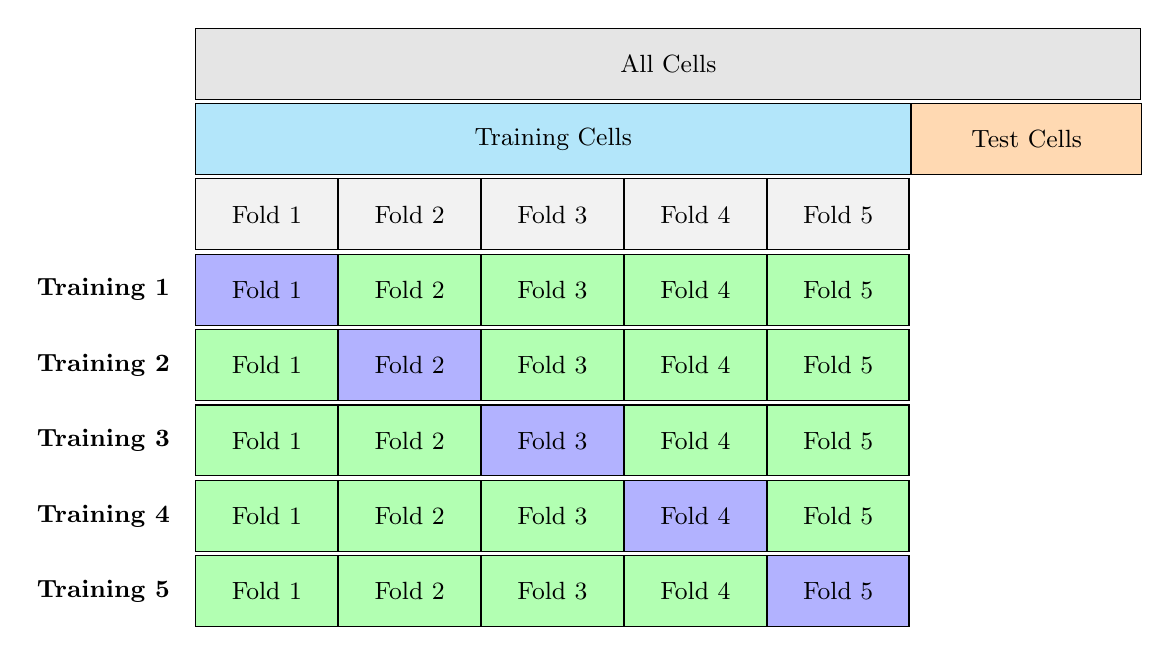
\begin{tikzpicture}[
    box/.style={rectangle, draw=black, minimum height=0.9cm, text centered, font=\small},
    fold/.style={rectangle, draw=black, minimum height=0.9cm, minimum width=1.8cm, text centered, font=\small},
    all_data/.style={box, fill=gray!20, minimum width=12cm},
    train_data/.style={box, fill=cyan!30, minimum width=9.075cm},
    test_data/.style={box, fill=orange!30, minimum width=2.925cm},
    foldtrain/.style={fold, fill=green!30},
    foldtest/.style={fold, fill=blue!30},
    legend/.style={font=\small\bfseries}
]
    % Top: Todos os dados
    \node[all_data] (all_data) {All Cells};
    % Segunda linha: divisão em treino e teste
    \node[train_data, below=0.5cm, at=(all_data.south west), anchor=west] (train_data) {Training Cells};
    \node[test_data, right=0cm, at=(train_data.east), anchor=west] (test_data) {Test Cells};
    % Terceira linha: cabeçalhos dos folds
    \node[fold, fill=gray!10, below=0.5cm, at=(train_data.south west), anchor=west] (foldh0) {Fold 1};
    \node[fold, fill=gray!10, right=0cm, at=(foldh0.east), anchor=west] (foldh1) {Fold 2};
    \node[fold, fill=gray!10, right=0cm, at=(foldh1.east), anchor=west] (foldh2) {Fold 3};
    \node[fold, fill=gray!10, right=0cm, at=(foldh2.east), anchor=west] (foldh3) {Fold 4};
    \node[fold, fill=gray!10, right=0cm, at=(foldh3.east), anchor=west] (foldh4) {Fold 5};
    
    % Validação cruzada com 5 linhas
    % Linha 1
    \node[legend, left=0.2cm, below=0.5cm, at=(foldh0.south west), anchor=east] (legend1) {Training 1};
    \node[foldtest, below=0.5cm, at=(foldh0.south west), anchor=west] (f11) {Fold 1};
    \node[foldtrain, right=0cm, at=(f11.east), anchor=west] (f12) {Fold 2};
    \node[foldtrain, right=0cm, at=(f12.east), anchor=west] (f13) {Fold 3};
    \node[foldtrain, right=0cm, at=(f13.east), anchor=west] (f14) {Fold 4};
    \node[foldtrain, right=0cm, at=(f14.east), anchor=west] (f15) {Fold 5};
    
    % Linha 2
    \node[legend, left=0.2cm, below=0.5cm, at=(f11.south west), anchor=east] (legend2) {Training 2};
    \node[foldtrain, below=0.5cm, at=(f11.south west), anchor=west] (f21) {Fold 1};
    \node[foldtest, right=0cm, at=(f21.east), anchor=west] (f22) {Fold 2};
    \node[foldtrain, right=0cm, at=(f22.east), anchor=west] (f23) {Fold 3};
    \node[foldtrain, right=0cm, at=(f23.east), anchor=west] (f24) {Fold 4};
    \node[foldtrain, right=0cm, at=(f24.east), anchor=west] (f25) {Fold 5};
    
    % Linha 3
    \node[legend, left=0.2cm, below=0.5cm, at=(f21.south west), anchor=east] (legend3) {Training 3};
    \node[foldtrain, below=0.5cm, at=(f21.south west), anchor=west] (f31) {Fold 1};
    \node[foldtrain, right=0cm, at=(f31.east), anchor=west] (f32) {Fold 2};
    \node[foldtest, right=0cm, at=(f32.east), anchor=west] (f33) {Fold 3};
    \node[foldtrain, right=0cm, at=(f33.east), anchor=west] (f34) {Fold 4};
    \node[foldtrain, right=0cm, at=(f34.east), anchor=west] (f35) {Fold 5};
    
    % Linha 4
    \node[legend, left=0.2cm, below=0.5cm, at=(f31.south west), anchor=east] (legend4) {Training 4};
    \node[foldtrain, below=0.5cm, at=(f31.south west), anchor=west] (f41) {Fold 1};
    \node[foldtrain, right=0cm, at=(f41.east), anchor=west] (f42) {Fold 2};
    \node[foldtrain, right=0cm, at=(f42.east), anchor=west] (f43) {Fold 3};
    \node[foldtest, right=0cm, at=(f43.east), anchor=west] (f44) {Fold 4};
    \node[foldtrain, right=0cm, at=(f44.east), anchor=west] (f45) {Fold 5};
    
    % Linha 5
    \node[legend, left=0.2cm, below=0.5cm, at=(f41.south west), anchor=east] (legend5) {Training 5};
    \node[foldtrain, below=0.5cm, at=(f41.south west), anchor=west] (f51) {Fold 1};
    \node[foldtrain, right=0cm, at=(f51.east), anchor=west] (f52) {Fold 2};
    \node[foldtrain, right=0cm, at=(f52.east), anchor=west] (f53) {Fold 3};
    \node[foldtrain, right=0cm, at=(f53.east), anchor=west] (f54) {Fold 4};
    \node[foldtest, right=0cm, at=(f54.east), anchor=west] (f55) {Fold 5};
\end{tikzpicture}
\caption{Diagram of data splitting in K-Fold cross-validation. On each training green folds are used to train, and the purple fold (validation set) is used to evaluate the trained model. Test cells are left out of the process.}
\label{fig:kfold}
\end{figure}